%%% LaTeX Template: Article/Thesis/etc. with colored headings and special fonts
%%%
%%% Source: http://www.howtotex.com/
%%% Feel free to distribute this template, but please keep to referal to http://www.howtotex.com/ here.
%%% February 2011
%%%
%%% Modified January 2016 by CDM

%%%  Preamble
\documentclass[11pt,letterpaper]{article}
\usepackage[margin=1.0in]{geometry}
\usepackage[T1]{fontenc}
\usepackage[bitstream-charter]{mathdesign}
\usepackage[latin1]{inputenc}					
\usepackage{amsmath}						
\usepackage{xcolor}
\usepackage{cite}
\usepackage{hyphenat}
\usepackage{graphicx}
\usepackage{float}
\usepackage{subfigure}
\usepackage{sectsty}
\usepackage[compact]{titlesec} 
\usepackage[tablegrid]{vhistory}
\usepackage{pbox}
\allsectionsfont{\color{accentcolor}\scshape\selectfont}

%%% Definitions
\definecolor{accentcolor}{rgb}{0.0,0.0,0.5} 
\newcommand{\teamname}{Team Hawt Wheels}
\newcommand{\productname}{Smart Cart}
\newcommand{\coursename}{CSE 4316: Senior Design I}
\newcommand{\semester}{Spring 2016}
\newcommand{\docname}{Architectural Design Specification}
\newcommand{\department}{Department of Computer Science \& Engineering}
\newcommand{\university}{The University of Texas at Arlington}
\newcommand{\authors}{David Harvey \\ Dennis Otieno \\ Peggy Soh \\ Brian Wong \\ Or Zoarets}

%%% Headers and footers
\usepackage{fancyhdr}
	\pagestyle{fancy}						% Enabling the custom headers/footers
\usepackage{lastpage}	
	% Header (empty)
	\lhead{}
	\chead{}
	\rhead{}
	% Footer
	\lfoot{\footnotesize \teamname \ - \semester}
	\cfoot{}
	\rfoot{\footnotesize page \thepage\ of \pageref{LastPage}}	% "Page 1 of 2"
	\renewcommand{\headrulewidth}{0.0pt}
	\renewcommand{\footrulewidth}{0.4pt}

%%% Change the abstract environment
\usepackage[runin]{abstract}			% runin option for a run-in title
%\setlength\absleftindent{30pt}			% left margin
%\setlength\absrightindent{30pt}		% right margin
\abslabeldelim{\quad}	
\setlength{\abstitleskip}{-10pt}
\renewcommand{\abstractname}{}
\renewcommand{\abstracttextfont}{\color{accentcolor} \small \slshape}	% slanted text

%%% Start of the document
\begin{document}

%%% Cover sheet
{\centering \huge \color{accentcolor} \sc \textbf{\department \\ \university} \par}
\vspace{1 in}
{\centering \huge \color{accentcolor} \sc \textbf{\docname \\ \coursename \\ \semester} \par}
\vspace{0.5 in}
\begin{figure}[h!]
	\centering
   	
\includegraphics[width=0.60\textwidth]{images/smart_cart}
\end{figure}
\vspace{0.5 in}
{\centering \huge \color{accentcolor} \sc \textbf{\teamname \\ \productname} \par}
\vspace{0.5 in}
{\centering \large \sc \textbf{\authors} \par}
\newpage


%\vspace{1 in}
%\centerline{January 13th, 2012}
%\newpage

%%% Revision History
\begin{versionhistory}
  	\vhEntry{0.1}{03.11.2016}{DH, DO, PS, BW, OZ}{Document creation}
  	\vhEntry{0.2}{04.08.2016}{DH, DO, PS, BW, OZ}{Complete draft}
\end{versionhistory}
\newpage

%%% Table of contents
\setcounter{tocdepth}{2}
\tableofcontents
\newpage

%%% List of figures and tables (optional)
\listoffigures
\listoftables
\newpage

%%% Document sections
\section{Introduction}
\subsection{Product Concept}
The Smart Cart will provide assistance by being an autonomous carrier. The cart needs to be able to do the following things:
\begin{itemize}
	\item Follow a ''master'' to the designated destination
	\item Avoid collision with obstacles such as walls and other people
	\item Include an integrated power supply
	\item Holonomic mobility
\end{itemize}

\subsection{Scope}
The main function of the Smart Cart is to help its user carry tools from one point to another. It will also have an integrated power supply to allow its user to charge or power his or her tools. A unique feature of the Smart Cart is that the cart will identify and follow its "master" by using the Intel RealSense. Another unique feature of the cart is its holonomic wheels. This allows the cart to easily maneuver and avoid collisions with objects by using image processing from a camera. The Smart Cart will require external input from the user. The user must wear a colored band that is provided with the Smart Cart. This band is used by the cart for tracking its "master". External outputs produced by the cart will be messages to let its user know whether it has succesfully identified its master. There are no other external inputs or outputs. A simple user interface may be implemented for identification of master depending on the availability of time. 

\subsection{Key Requirements}
The Smart Cart shall have five layers that work in unison to allow the cart to autonomously navigate and follow a specified user. The five layers in the system are the Smart Cart layer, Power Supply layer, Imaging/Navigation layer and Crab Drive layer. The five layers will be discussed more in the following sections.
\newpage
\section{System Overview}
This section should describe the overall structure of your software system. Think of it as the strategy for how you will build the system. An architectural "layer" is the top-level logical view, or an abstraction, of your design. Layers should be composed of related elements of similar capabilities, and should be highly independent of other layers, but should have very clearly defined interfaces and interactions with other layers. Each layer should be identified individually and should be unique as to its function and purpose within the system. This section should also contain the high-level block diagram of the layers, as shown in the example below, as well as detailed descriptions of the functions of each layer.

\begin{figure}[h!]
	\centering
 	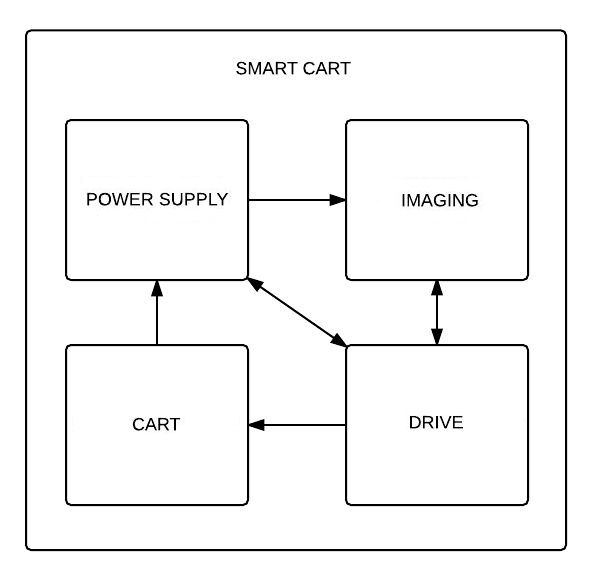
\includegraphics[width=0.60\textwidth]{images/system_overview}
 \caption{A simple architectural layer diagram}
\end{figure}


\subsection{Power Supply Layer Description}
Each layer should be described separately in detail. Descriptions should include the features, functions, critical interfaces and interactions of the layer. The description should clearly define the services that the layer provides. Also include any conventions that your team will use in describing the structure: naming conventions for layers, subsystems, modules, and data flows; interface specifications; how layers and subsystems are defined; etc.

\subsection{Cart Layer Description}
Each layer should be described separately in detail. Descriptions should include the features, functions, critical interfaces and interactions of the layer. The description should clearly define the services that the layer provides. Also include any conventions that your team will use in describing the structure: naming conventions for layers, subsystems, modules, and data flows; interface specifications; how layers and subsystems are defined; etc.

\subsection{Crab Drive Layer Description}
Each layer should be described separately in detail. Descriptions should include the features, functions, critical interfaces and interactions of the layer. The description should clearly define the services that the layer provides. Also include any conventions that your team will use in describing the structure: naming conventions for layers, subsystems, modules, and data flows; interface specifications; how layers and subsystems are defined; etc. 

\subsection{Imaging and Navigation Description}
Each layer should be described separately in detail. Descriptions should include the features, functions, critical interfaces and interactions of the layer. The description should clearly define the services that the layer provides. Also include any conventions that your team will use in describing the structure: naming conventions for layers, subsystems, modules, and data flows; interface specifications; how layers and subsystems are defined; etc. 
\newpage
\section{Subsystem Definitions \& Data Flow}
This section breaks down the simple architectural layer diagram with another level of detail. The logical subsystems that compose each layer and its interactions and interfaces between the subsystems are graphically represented. Even though the power supply layer does not have data flow, it is still a key layer to the system. The following data flow block diagram shows a high level diagram of all the layers in the Smart Cart.

\begin{figure}[h!]
	\centering
 	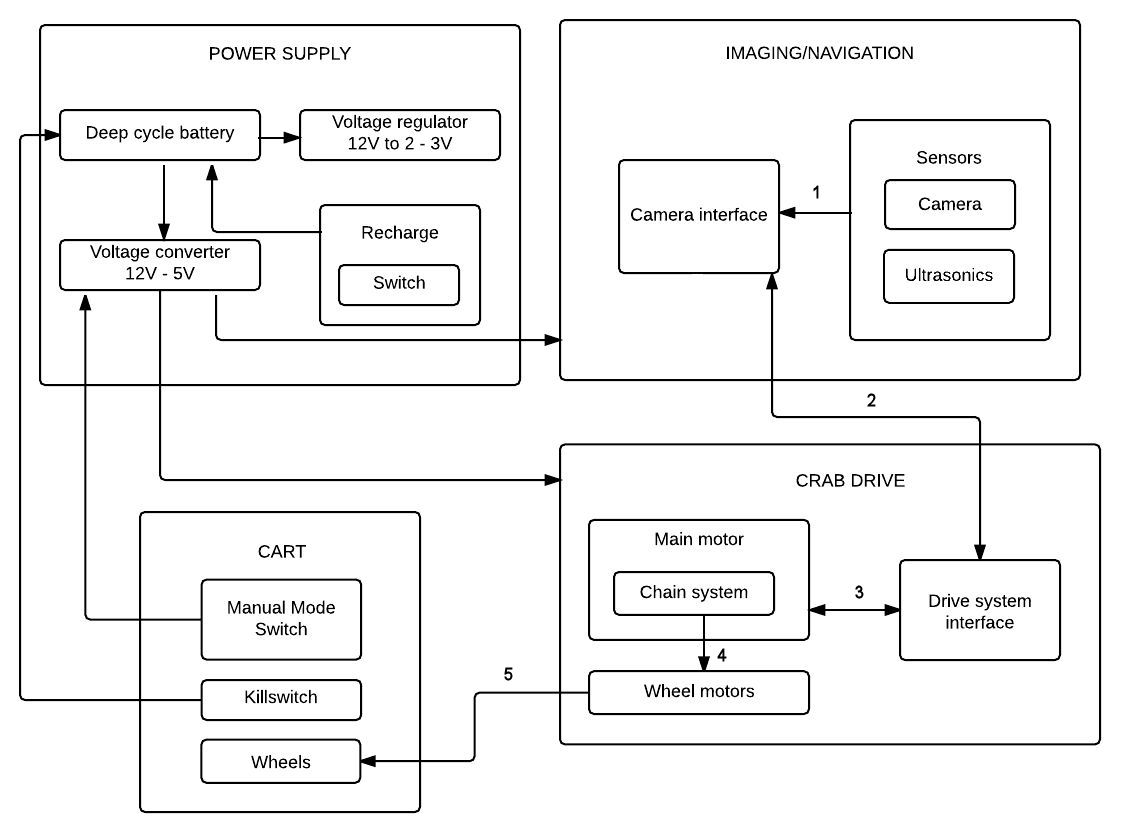
\includegraphics[width=\textwidth]{images/diagram_whole}
 \caption{A simple data flow diagram}
\end{figure}

\newpage
\section{Power Supply Subsystems}
The power supply layer is one if not the most important layer because it provides stable power supply to the cart. The parts in this subsystem are responsible for powering every other subsystem and any external tools or equiment. 

\begin{figure}[h!]
	\centering
 	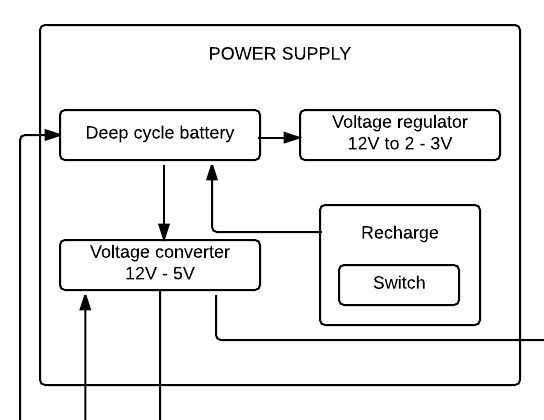
\includegraphics[width=0.60\textwidth]{images/power_supply}
 \caption{Power supply layer}
\end{figure}

\subsection{Deep Cycle Battery}
The deep cycle battery is designed to power everything. Once the cart's switch is turned on, the deep cycle battery will then begin to power the other subsystems on.

\begin{figure}[h!]
	\centering
 	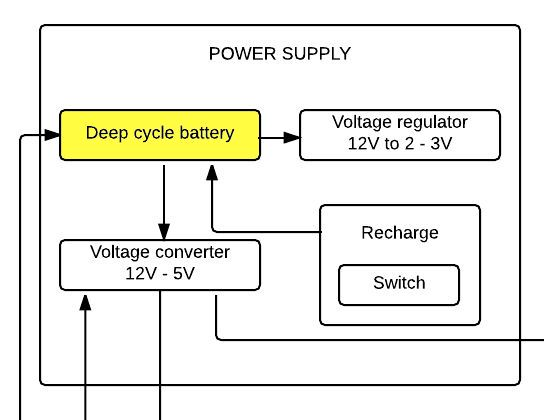
\includegraphics[width=0.60\textwidth]{images/power_supply_batt}
 \caption{Deep cycle battery subsystem}
\end{figure}

\subsubsection{Assumptions}
Assumptions made are as follows:
\begin{itemize}
	\item The battery is charged.
	\item The battery is properly connected to the cart.
	\item The battery is fully functional.
	\item The battery is connected to the cart at all times.
	\item The battery will be 12V.
\end{itemize}

\subsubsection{Responsibilities}
The deep cycle battery subsystem's responsibilities are as follows:
\begin{itemize}
	\item Enable stable power to the other subsystems after being converted from 12V to 5V through the voltage converter.
	\item Enable stable power to external tools and equipment after being converted from 12V to 2 - 3V through the voltage regulator.
\end{itemize}

\subsubsection{Subsystem Interfaces}

\begin {table}[H]
\caption {Deep cycle battery subsystem interfaces} 
\begin{center}
    \begin{tabular}{ | p{1cm} | p{6cm} | p{3cm} | p{3cm} |}
    \hline
    ID & Description & Inputs & Outputs \\ \hline
    \ N/A & Power integrated power supply & \pbox{3cm}{N/A} & \pbox{3cm}{Voltage regulator }  \\ \hline
    \ N/A & Power electronic components & \pbox{3cm}{N/A} & \pbox{3cm}{Voltage converter}  \\ \hline
    \ N/A & Safety killswitch & \pbox{3cm}{Killswitch} & \pbox{3cm}{N/A}  \\ \hline
    \ N/A & Safety manual mode & \pbox{3cm}{Manual-mode switch} & \pbox{3cm}{N/A}  \\ \hline
    \end{tabular}
\end{center}
\end{table}

\subsection{Voltage Regulator}
The voltage regulator is designed to convert the 12V voltage from the deep cycle battery to 2 - 3V and it will mainly be used to power up external tools and equipment.

\begin{figure}[h!]
	\centering
 	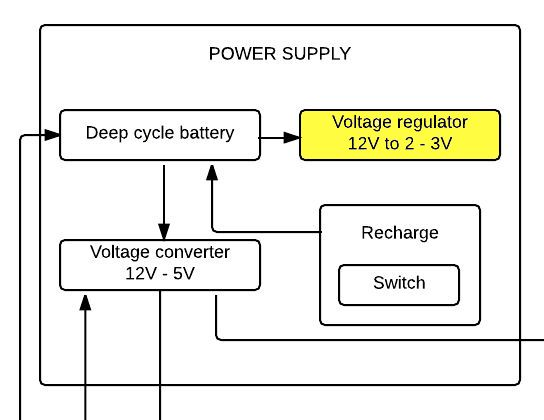
\includegraphics[width=0.60\textwidth]{images/power_supply_regulator}
 \caption{Voltage regulator subsystem}
\end{figure}

\subsubsection{Assumptions}
Assumptions made are as follows:
\begin{itemize}
	\item The voltage from the battery will be 12V.
	\item The voltage required for external tools and equipment will be between 2 - 3V.
\end{itemize}

\subsubsection{Responsibilities}
The voltage regulator subsystem's responsibilities are as follows:
\begin{itemize}
	\item To enable and regulate constant voltage level for powering external tools and supplies.
\end{itemize}

\subsubsection{Subsystem Interfaces}
\begin {table}[H]
\caption {Voltage regulator subsystem interfaces} 
\begin{center}
    \begin{tabular}{ | p{1cm} | p{6cm} | p{3cm} | p{3cm} |}
    \hline
    ID & Description & Inputs & Outputs \\ \hline
    \ N/A & Receive power & \pbox{3cm}{Deep cycle battery} & \pbox{3cm}{N/A}  \\ \hline
    \end{tabular}
\end{center}
\end{table}
\newline

\subsection{Voltage Converter}
The voltage regulator is designed to convert the 12V voltage from the deep cycle battery to 2 - 3V and it will mainly be used to power up the Smart Cart's components.

\begin{figure}[h!]
	\centering
 	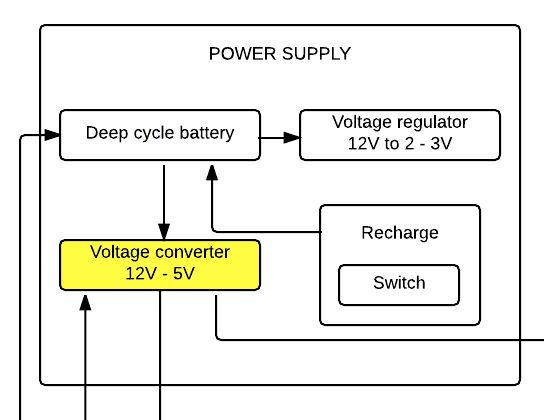
\includegraphics[width=0.60\textwidth]{images/power_supply_converter}
 \caption{Voltage converter subsystem}
\end{figure}

\subsubsection{Assumptions}
Assumptions made are as follows:
\begin{itemize}
	\item The voltage from the battery will be 12V.
	\item The voltage required for the cart's components will be 5V.
\end{itemize}

\subsubsection{Responsibilities}
The voltage converter subsystem's responsibilities are as follows:
\begin{itemize}
	\item Enable stable power to the other subsystems, which include the crab drive system and image processing after being converted from 12V to 5V through the voltage converter.
\end{itemize}

\subsubsection{Subsystem Interfaces}
\begin {table}[H]
\caption {Voltage converter subsystem interfaces} 
\begin{center}
    \begin{tabular}{ | p{1cm} | p{6cm} | p{3cm} | p{3cm} |}
    \hline
    ID & Description & Inputs & Outputs \\ \hline
    \ N/A & Receive power & \pbox{3cm}{Deep cycle battery} & \pbox{3cm}{N/A}  \\ \hline
    \ N/A & Safety manual mode & \pbox{3cm}{Manual-mode switch} & \pbox{3cm}{Crab-drive system \\ Imaging and navigation}  \\ \hline
    \end{tabular}
\end{center}
\end{table}
\newline

\subsection{Recharge}
The recharge subsystem will be used to ensure that the Smart Cart will be charged without having too much electricity going to the electronics or the other battery and cause problems.

\begin{figure}[h!]
	\centering
 	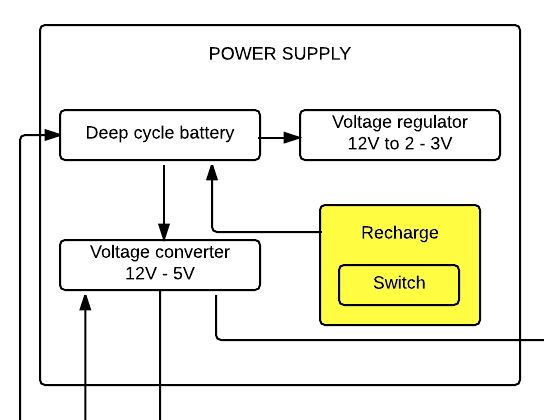
\includegraphics[width=0.60\textwidth]{images/power_supply_recharge}
 \caption{Recharge subsystem}
\end{figure}

\subsubsection{Assumptions}
Assumptions made are as follows:
\begin{itemize}
	\item The recharge subsystem will ensure the safety of the tools and equipment.
\end{itemize}

\subsubsection{Responsibilities}
The recharge subsystem's responsibilities are as follows:
\begin{itemize}
	\item A switch will disable the battery from powering the Smart Cart components while it is being recharged.
\end{itemize}

\subsubsection{Subsystem Interfaces}
\begin {table}[H]
\caption {Recharge subsystem interfaces} 
\begin{center}
    \begin{tabular}{ | p{1cm} | p{6cm} | p{3cm} | p{3cm} |}
    \hline
    ID & Description & Inputs & Outputs \\ \hline
    \ N/A & Switch on safety & \pbox{3cm}{Switch} & \pbox{3cm}{Deep cycle battery}  \\ \hline
    \end{tabular}
\end{center}
\end{table}
\newpage
\section{Cart Subsystems}
The cart layer consists of the hardware components of the cart as well as the switches. The switches include a manual mode switch to remove autonomous activity and a killswitch to immediately unpower the cart.

\begin{figure}[h!]
	\centering
 	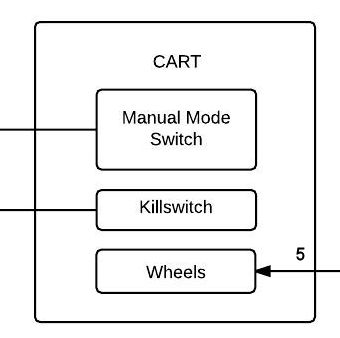
\includegraphics[width=0.60\textwidth]{images/cart}
 \caption{Cart layer}
\end{figure}

\subsection{Manual Mode Switch}
The manual mode switch subsystem will be used to ensure that the Smart Cart will not be autonomously moving.

\begin{figure}[h!]
	\centering
 	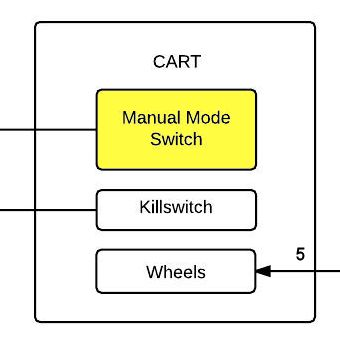
\includegraphics[width=0.60\textwidth]{images/cart_manual}
 \caption{Manual mode switch subsystem}
\end{figure}

\subsubsection{Assumptions}
Assumptions made are as follows:
\begin{itemize}
	\item The manual mode switch subsystem will ensure the safety of the users and people around the user.
	\item The manual mode switch subsystem will not power the Smart Cart off, but simply disable autnomous smovement.
\end{itemize}

\subsubsection{Responsibilities}
The manual mode switch subsystem's responsibilities are as follows:
\begin{itemize}
	\item The switch will disable the autonomous movement of the cart.
	\item The switch will ensure the safety of the user and surrounding people.
\end{itemize}

\subsubsection{Subsystem Interfaces}

\begin {table}[H]
\caption {Manual mode switch subsystem interfaces} 
\begin{center}
    \begin{tabular}{ | p{1cm} | p{6cm} | p{3cm} | p{3cm} |}
    \hline
    ID & Description & Inputs & Outputs \\ \hline
    \ N/A & Disable converter & \pbox{3cm}{N/A} & \pbox{3cm}{Voltage converter}  \\ \hline
    \end{tabular}
\end{center}
\end{table}
\newline


\subsection{Killswitch}
The killswitch subsystem will be used to ensure that the Smart Cart will be immediately turned off.

\begin{figure}[h!]
	\centering
 	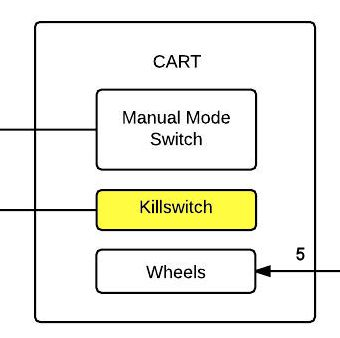
\includegraphics[width=0.60\textwidth]{images/cart_kill}
 \caption{Killswitch subsystem}
\end{figure}

\subsubsection{Assumptions}
Assumptions made are as follows:
\begin{itemize}
	\item Power to the Smart Cart components will be disabled.
	\item Power to external tools and equipment will be disabled.
\end{itemize}

\subsubsection{Responsibilities}
The killswitch subsystem's responsibilities are as follows:
\begin{itemize}
	\item The switch will disable the battery from powering the Smart Cart and its components.
\end{itemize}

\subsubsection{Subsystem Interfaces}

\begin {table}[H]
\caption {Killswitch subsystem interfaces} 
\begin{center}
    \begin{tabular}{ | p{1cm} | p{6cm} | p{3cm} | p{3cm} |}
    \hline
    ID & Description & Inputs & Outputs \\ \hline
    \ N/A & Disable battery & \pbox{3cm}{N/A} & \pbox{3cm}{Deep cycle battery}  \\ \hline
    \end{tabular}
\end{center}
\end{table}
\newline


\subsection{Wheels}
The wheels subsystem will be used to provide movement to the Smart Cart. The wheels will be controlled by the Crab Drive layer.

\begin{figure}[h!]
	\centering
 	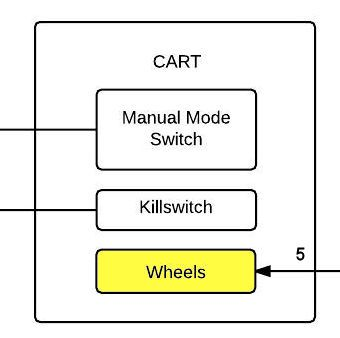
\includegraphics[width=0.60\textwidth]{images/cart_wheel}
 \caption{Wheels subsystem}
\end{figure}

\subsubsection{Assumptions}
Assumptions made are as follows:
\begin{itemize}
	\item The wheels must be able to turn in any sort of direction.
	\item The wheels will move together as a whole.
\end{itemize}

\subsubsection{Responsibilities}
The wheels subsystem's responsibilities are as follows:
\begin{itemize}
	\item The wheels will be able to withstand movement through rough terrain.
	\item The wheels' movement and direction will be controlled by the wheel motors.
\end{itemize}

\subsubsection{Subsystem Interfaces}

\begin {table}[H]
\caption {Wheel subsystem interfaces} 
\begin{center}
    \begin{tabular}{ | p{1cm} | p{6cm} | p{3cm} | p{3cm} |}
    \hline
    ID & Description & Inputs & Outputs \\ \hline
    \#5 & Move wheels & \pbox{3cm}{Wheel motors} & \pbox{3cm}{N/A}  \\ \hline
    \end{tabular}
\end{center}
\end{table}

\newpage
\section{Crab Drive Subsystems}
The crab drive layer consists of the hardware components that include a main drive motor that is responsible for steering the wheel motors that move the wheels. The drive system interface is responsible for communicating with the camera interface in the imaging subsystem, supplying directions to the main motor, and providing the cart with holonomic capabilities.

\begin{figure}[h!]
	\centering
 	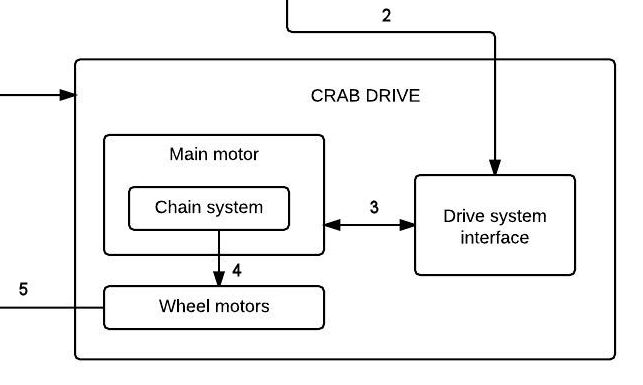
\includegraphics[width=0.60\textwidth]{images/crab}
 \caption{Crab drive layer}
\end{figure}

\subsection{Drive System Interface Subsystem}
The drive system interface is designed to communicate with the navigation subsystem's camera interface. it will get  navigation data from the camera interface to steer the main drive motor as well as receiving feedback information for the wheel orientations.

\begin{figure}[h!]
	\centering
 	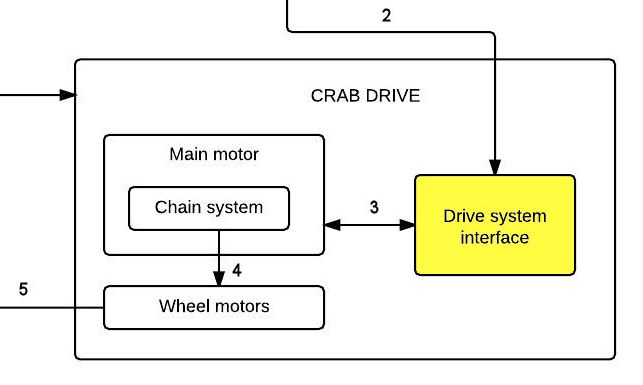
\includegraphics[width=0.60\textwidth]{images/crab_interface}
 \caption{Drive system interface subsystem}
\end{figure}

\subsubsection{Assumptions}
Assumptions made are as follows:
\begin{itemize}
	\item The drive system interface will receive accurate navigation data from the camera interface.
	\item The drive system interface will receive accurate feedback data from the main motor about wheel orientation.
\end{itemize}

\subsubsection{Responsibilities}
The drive system interface subsystem's responbilities are as follows:
\begin{itemize}
	\item Send navigation data to the main motor.
	\item Receive wheel feedback data.
\end{itemize}

\subsubsection{Subsystem Interfaces}

\begin {table}[H]
\caption {Drive system interface subsystem interfaces} 
\begin{center}
    \begin{tabular}{ | p{1cm} | p{6cm} | p{3cm} | p{3cm} |}
    \hline
    ID & Description & Inputs & Outputs \\ \hline
    \#2 & Receive navigation data  & \pbox{3cm}{Camera interface} & \pbox{3cm}{Main motor}  \\ \hline
    \#3 & Receive wheel data & \pbox{3cm}{Main motor} & \pbox{3cm}{Camera interface}  \\ \hline
    \end{tabular}
\end{center}
\end{table}
\newline


\subsection{Main Motor Subsystem}
The main motor will contain a chain system that is responsible for steering the cart and maintaining a consistent orientation for all of the wheels.

\begin{figure}[h!]
	\centering
 	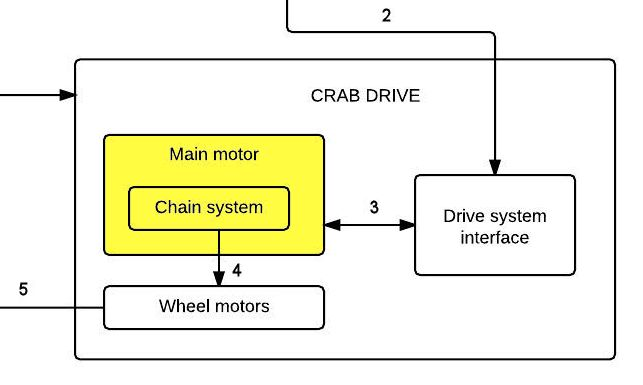
\includegraphics[width=0.60\textwidth]{images/crab_motor}
 \caption{Main motor subsystem}
\end{figure}

\subsubsection{Assumptions}
Assumptions made are as follows:
\begin{itemize}
	\item The main motor will correctly steer the wheels with the chain/belt system.
	\item The main motor will have a method to accurately keep wheel orientation data.
\end{itemize}

\subsubsection{Responsibilities}
The main motor subsystem's responbilities are as follows:
\begin{itemize}
	\item Receive steering instructions from the drive system interface and accurately perform instructions.
\end{itemize}

\subsubsection{Subsystem Interfaces}

\begin {table}[H]
\caption {Main motor subsystem interfaces} 
\begin{center}
    \begin{tabular}{ | p{1cm} | p{6cm} | p{3cm} | p{3cm} |}
    \hline
    ID & Description & Inputs & Outputs \\ \hline
    \#4 & Steer wheels  & \pbox{3cm}{Drive system interface} & \pbox{3cm}{Wheel motors}  \\ \hline
    \#3 & Feedback data  & \pbox{3cm}{N/A} & \pbox{3cm}{Drive system interface}  \\ \hline
    \end{tabular}
\end{center}
\end{table}
\newline


\subsection{Wheel Motors Subsystem}
The wheel motors is designed to drive the wheels at an appropriate speed to follow the user using information sent by the main motor.

\begin{figure}[h!]
	\centering
 	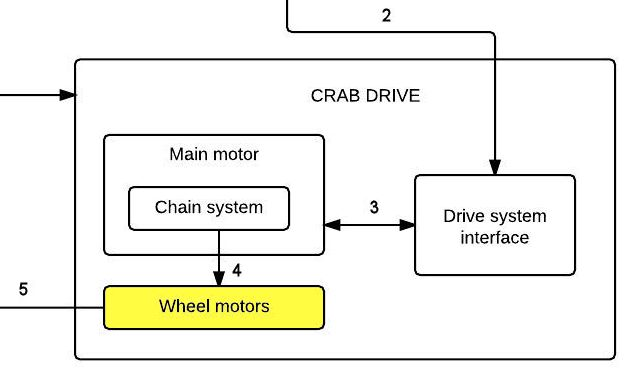
\includegraphics[width=0.60\textwidth]{images/crab_wheel}
 \caption{Wheel motors subsystem}
\end{figure}

\subsubsection{Assumptions}
Assumptions made are as follows:
\begin{itemize}
	\item The wheel motors will be able to decide how fast to spin to achieve an appropriate speed.
	\item The wheel motors will only spin in one direction as the chain/belt system will control steering.
\end{itemize}

\subsubsection{Responsibilities}
The wheel motors subsystem's responbilities are as follows:
\begin{itemize}
	\item Drive the wheels to follow a user at an appropriate speed.
\end{itemize}

\subsubsection{Subsystem Interfaces}

\begin {table}[H]
\caption {Wheel motors subsystem interfaces} 
\begin{center}
    \begin{tabular}{ | p{1cm} | p{6cm} | p{3cm} | p{3cm} |}
    \hline
    ID & Description & Inputs & Outputs \\ \hline
    \#5 & Receive drive data  & \pbox{3cm}{Chain system} & \pbox{3cm}{Wheels}  \\ \hline
    \end{tabular}
\end{center}
\end{table}
\newpage
\section{Imaging and Navigation Subsystems}
The imaging and navigation layer consists of the Intel Realsense camera, ultrasonic sensors, and imaging software to produce navigation data to be sent to the drive system interface. The navigation data that will direct the crab drive system to follow a user as well as obstacle avoidance.

\begin{figure}[h!]
	\centering
 	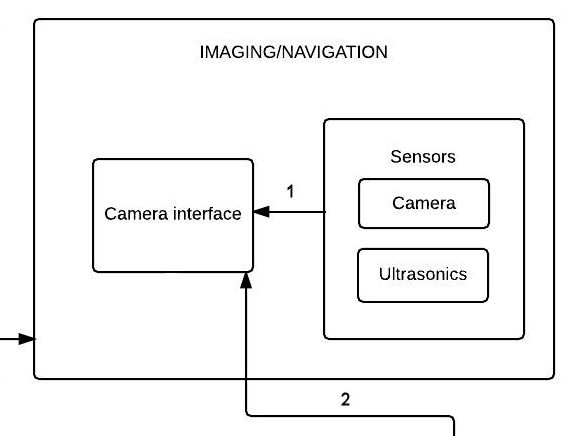
\includegraphics[width=0.60\textwidth]{images/imaging}
 \caption{Imaging and navigation layer}
\end{figure}

\subsection{Sensors Subsystem}
Sensors include the Intel RealSense camera and ultrasonic sensors. The RealSense will identify a user to follow and the ultrasonic sensors will be used for obstacle avoidance. The sensors will provide the necessary information to the camera interface needed to create navigation data.

\begin{figure}[h!]
	\centering
 	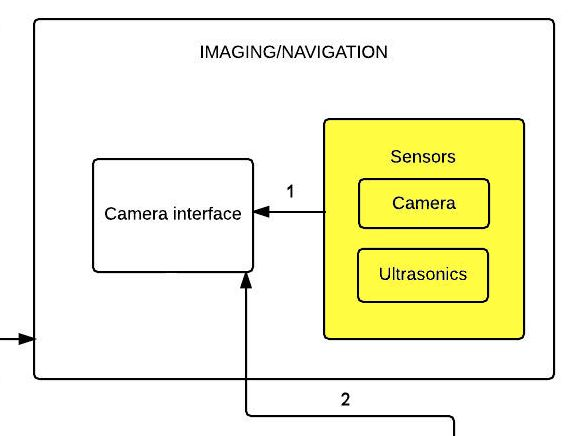
\includegraphics[width=0.60\textwidth]{images/imaging_sensors}
 \caption{Sensors subsystem}
\end{figure}

\subsubsection{Assumptions}
Assumptions made are as follows:
\begin{itemize}
	\item The user will be wearing a colored wristband that identifies them as the master.
	\item The user will stay in front of the Intel RealSense to avoid possible errors, such as the cart losing vision of its master.
\end{itemize}

\subsubsection{Responsibilities}
The sensor subsystem's responsibilities are as follows:
\begin{itemize}
	\item Process image and ultrasonic data in real time.
	\item Keep the designated master within the image frame.
	\item Gather accurate data to send to the camera interface.
\end{itemize}

\subsubsection{Subsystem Interfaces}

\begin {table}[H]
\caption {Sensors subsystem interfaces} 
\begin{center}
    \begin{tabular}{ | p{1cm} | p{6cm} | p{3cm} | p{3cm} |}
    \hline
    ID & Description & Inputs & Outputs \\ \hline
    \#1 & Send sensor data & \pbox{3cm}{Camera \\ Ultrasonics} & \pbox{3cm}{Camera interface}  \\ \hline
    \end{tabular}
\end{center}
\end{table}
\newline


\subsection{Camera Interface Subsystem}
The camera interface is responsible for taking the data received from sensors to calculate accurate navigation data to send to the crab drive's drive system interface. The navigation data will include required speed, direction needed, and cart position for collision avoidance.

\begin{figure}[h!]
	\centering
 	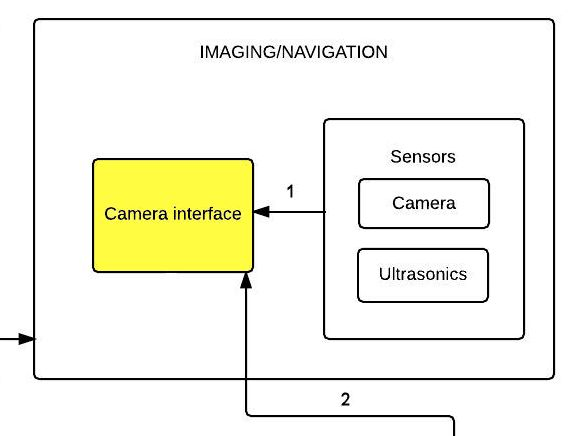
\includegraphics[width=0.60\textwidth]{images/imaging_camera}
 \caption{Camera interface subsystem}
\end{figure}

\subsubsection{Assumptions}
Assumptions made are as follows:
\begin{itemize}
	\item Accurate data is being sent from the sensors.
	\item The camera interface will be able to communicate with the drive system interface.
\end{itemize}

\subsubsection{Responsibilities}
The camera interface subsystem's responsibilities are as follows:
\begin{itemize}
	\item Calculate and process navigation data.
	\item Communicate necessary information to the drive system interface.
\end{itemize}

\subsubsection{Subsystem Interfaces}

\begin {table}[H]
\caption {Camera interface subsystem interfaces} 
\begin{center}
    \begin{tabular}{ | p{1cm} | p{6cm} | p{3cm} | p{3cm} |}
    \hline
    ID & Description & Inputs & Outputs \\ \hline
    \#2 & Calculate navigation data & \pbox{3cm}{Sensors} & \pbox{3cm}{Drive system interface}  \\ \hline
    \end{tabular}
\end{center}
\end{table}

\newpage

%%% References
\bibliographystyle{plain}
\bibliographystyle{reference/IEEEtran_custom}
\bibliography{reference/refs}{}

\end{document}